\section{Architecture}
\begin{figure}[tbh]
    \centering
    
\includegraphics[width=0.8\textwidth]{figures/overview.png}
    \caption{The overview of \method. \method adpots the Thinker-Talker architecture. Thinker is tasked with text generation while Talker focuses on generating streaming speech tokens by receives high-level representations directly from Thinker.}
    \label{fig:ovewview_arch}
\end{figure}

\subsection{Overview}
As shown in Figure~\ref{fig:ovewview_arch}, \method employs Thinker-Talker architecture. Thinker functions like a brain, responsible for processing and understanding inputs from text, audio and video modalities, generating high-level representations and corresponding text. Talker operates like a human mouth, taking in the high-level representations and text produced by the Thinker in a streaming manner, and outputting discrete tokens of speech fluidly. Thinker is a Transformer decoder, accompanied by encoders for audio and image that facilitate information extraction. In contrast, Talker is designed as a dual-track autoregressive Transformer Decoder architecture, motivated by Mini-Omni~\citep{xie2024mini}. During both training and inference, Talker directly receives high-dimensional representations from Thinker and shares all of Thinker's historical context information. Consequently, the entire architecture operates as a cohesive single model, enabling end-to-end training and inference.

In the following sections, we first introduce how \method perceives various input signals and present our proposed novel positional encoding algorithm, TMRoPE. Subsequently, the details of text and speech generation are presented. Finally, we highlight the improvements made in the understanding and generation modules to facilitate efficient streaming inference.


\subsection{Perceivation}
\begin{figure}[tbh]
    \centering
    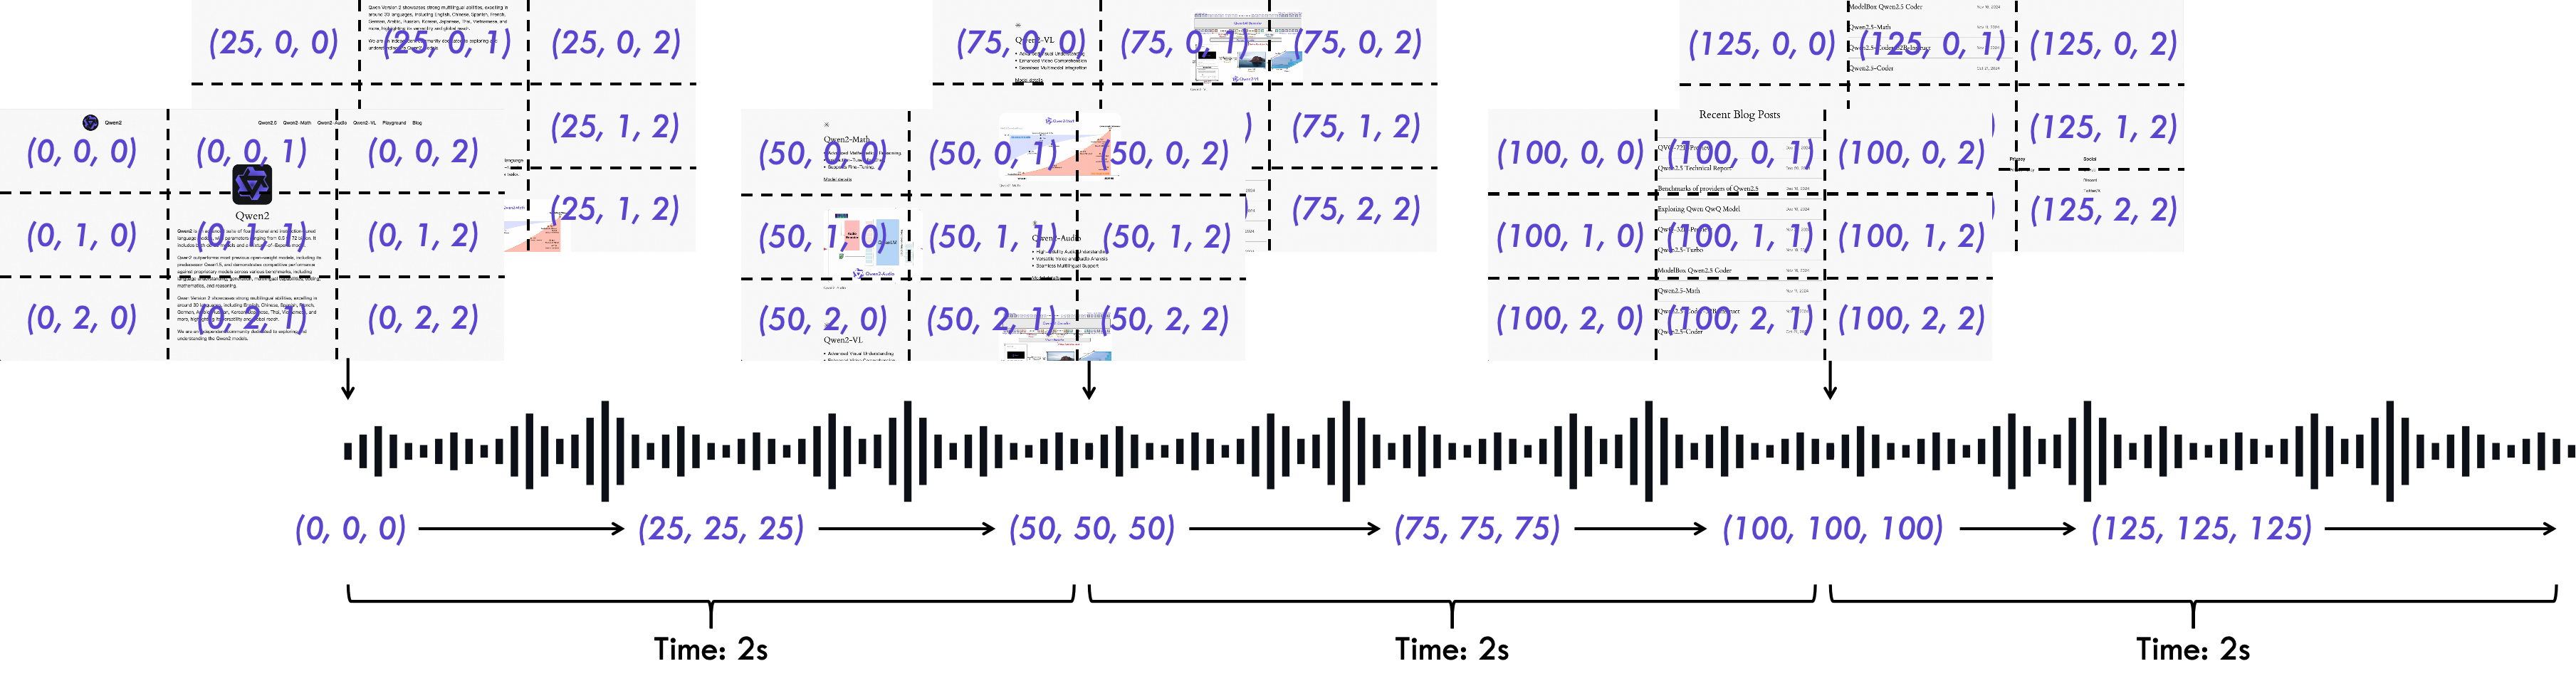
\includegraphics[width=1.0\textwidth]{figures/ATMRoPE.png}
    \caption{An illustration of Time-aligned Multimodal RoPE~(TMRoPE).}
    \label{fig:ATMRoPE}
\end{figure}
\paragraph{Text, Audio, Image and Video (w/o Audio).} Thinker processes text, audio, images, and video~(without the audio track) by converting them into a series of hidden representations for input. For tokenizing text, we use Qwen's tokenizer~\citep{qwen2}, which applies byte-level byte-pair encoding with a vocabulary comprising 151,643 regular tokens. Regarding audio input and audio from videos, we resample it to a frequency of 16kHz and transform the raw waveform into a 128-channel mel-spectrogram with a window size of 25ms and a hop size of 10ms. We adopt the audio encoder from Qwen2-Audio~\citep{qwen2-audio}, to make each frame of audio representation roughly corresponds to a 40ms segment of the original audio signal. Furthermore, we employ the vision encoder from Qwen2.5-VL~\citep{bai2025qwen25}, which is based on the Vision Transformer (ViT) model with approximately 675 million parameters, enabling it to effectively handle both image and video inputs. The vision encoder employs a mixed training regimen incorporating both image and video data, ensuring proficiency in image understanding and video comprehension. To preserve video information as completely as possible while adapting to the audio sampling rate, we sample the video using a dynamic frame rate. Additionally, for consistency, each image is treated as two identical frames.

\paragraph{Video and TMRoPE.} 
We propose a time-interleaving algorithm for audio and video, along with a novel position encoding approach. As shown in Figure~\ref{fig:ATMRoPE}, TMRoPE encodes the 3-D positional information of multimodal inputs, which is Multimodal Rotary Position Embedding (M-RoPE)~\citep{qwenvl} with absolute temporal positions. This is achieved by deconstructing the original rotary embedding into three components: temporal, height, and width. For text inputs, these components utilize identical position IDs, making M-RoPE functionally equivalent to 1D-RoPE. Similarly, for audio inputs, we also use identical position IDs and introduce absolute temporal position encoding, with one temporal ID corresponding to 40ms.

When processing images, the temporal IDs of each visual token remain constant, while distinct IDs are assigned to the height and width components based on the token’s position in the image. When the input is video with audio, the audio is still encoded with identical position IDs for every 40ms per frame, and the video is treated as a series of images with temporal ID increments for each frame, while the height and width components follow the same ID assignment pattern as images. Since the frame rate in video is not fixed, we dynamically adjust the temporal IDs between frames based on the actual time corresponding to each frame to ensure that one temporal ID corresponds to 40ms. In scenarios where the model’s input encompasses multiple modalities, position numbering for each modality is initialized by incrementing the maximum position ID of the preceding modality by one. TMRoPE enhances positional information modeling, maximizing the integration of various modalities, enabling \method to simultaneously understand and analyze information from multiple modalities.

After incorporating positional information into each modality, we arrange the representations in order. To enable the model to receive both visual and auditory information simultaneously, as shown in Figure~\ref{fig:ATMRoPE}, we have a special design for video with audio called the time-interleaving method, which segments the representation in the video with audio into chunks every 2 seconds according to the actual time. We then arrange the visual representation at the front and the audio representation at the back within the 2 seconds, interleaving the representations of the video with audio.

\subsection{Generation}
\paragraph{Text.} Text is generated directly by Thinker. The logic of text generation is fundamentally the same as that employed by widely used LLMs, which generate text through autoregressive sampling based on the probability distribution over the vocabulary. The generation process may incorporate techniques such as repetition penalty and top-p sampling to enhance its diversity.

\paragraph{Speech.} Talker receives both high-level representations and embeddings of the text tokens sampled by Thinker. The integration of high-dimensional representations and discrete sampling tokens is essential in this context. As a streaming algorithm, voice generation must anticipate the content's tone and attitude before the entire text is fully generated. The high-dimensional representations provided by Thinker implicitly convey this information, enabling a more natural streaming generation process. Furthermore, Thinker's representations primarily express semantic similarity in the representational space rather than phonetic similarity. Consequently, even phonetically distinct words may have very similar high-level representations, necessitating the input of sampled discrete tokens to eliminate such uncertainty.

We designed an efficient speech codec named \textit{qwen-tts-tokenizer}. \textit{qwen-tts-tokenizer} efficiently represents key information of speech and can be decoded to speech streamingly through a causal audio decoder. After receiving the information, Talker starts to autoregressively generate audio tokens and text tokens. The generation of speech does not require word-level and timestamp-level alignment with the text. This significantly simplifies the requirements for training data and the inference process.

\subsection{Designs for Streaming}
In the context of streaming audio and video interactions, the initial packet latency is a critical indicator of the system's streaming performance. This latency is influenced by several factors: 1) the delay caused by the processing of multimodal information inputs; 2) the latency from the moment the first text input is received until the first voice token is output; 3) the delay in converting the first segment of speech into audio; and 4) the inherent latency of the architecture itself, which is related to model size, computational FLOPs, and other factors. This paper will subsequently discuss the algorithmic and architectural improvements made to reduce these latencies across these four dimensions.

\paragraph{Support Prefilling.} Chunked-prefills is a mechanism widely used in modern inference framework. To support it in modalities interation, we modified the audio and visual encoders to support block-wise attention along the temporal dimension. Specifically, the audio encoder is changed from full attention over the entire audio to performing attention in blocks of 2 seconds each. The vision encoder utilizes flash attention for efficient training and inference with a simple MLP layer that merges adjacent 2×2 tokens into a single token. The patch size is set to 14, which allows images of different resolutions to be packed into a sequence.

\paragraph{Streaming Codec Generation.} To facilitate the streaming of audio, especially for extended sequences, we propose a sliding window block attention mechanism that restricts the current token's access to a limited context. Specifically, we utilize a Flow-Matching~\citep{flowmatching} DiT model. The input code is transformed into a mel-spectrogram using Flow-Matching, followed by a modified BigVGAN~\citep{sangbigvgan} to reconstruct the generated mel-spectrogram back into the waveform.

\begin{figure}[h]
    \centering
    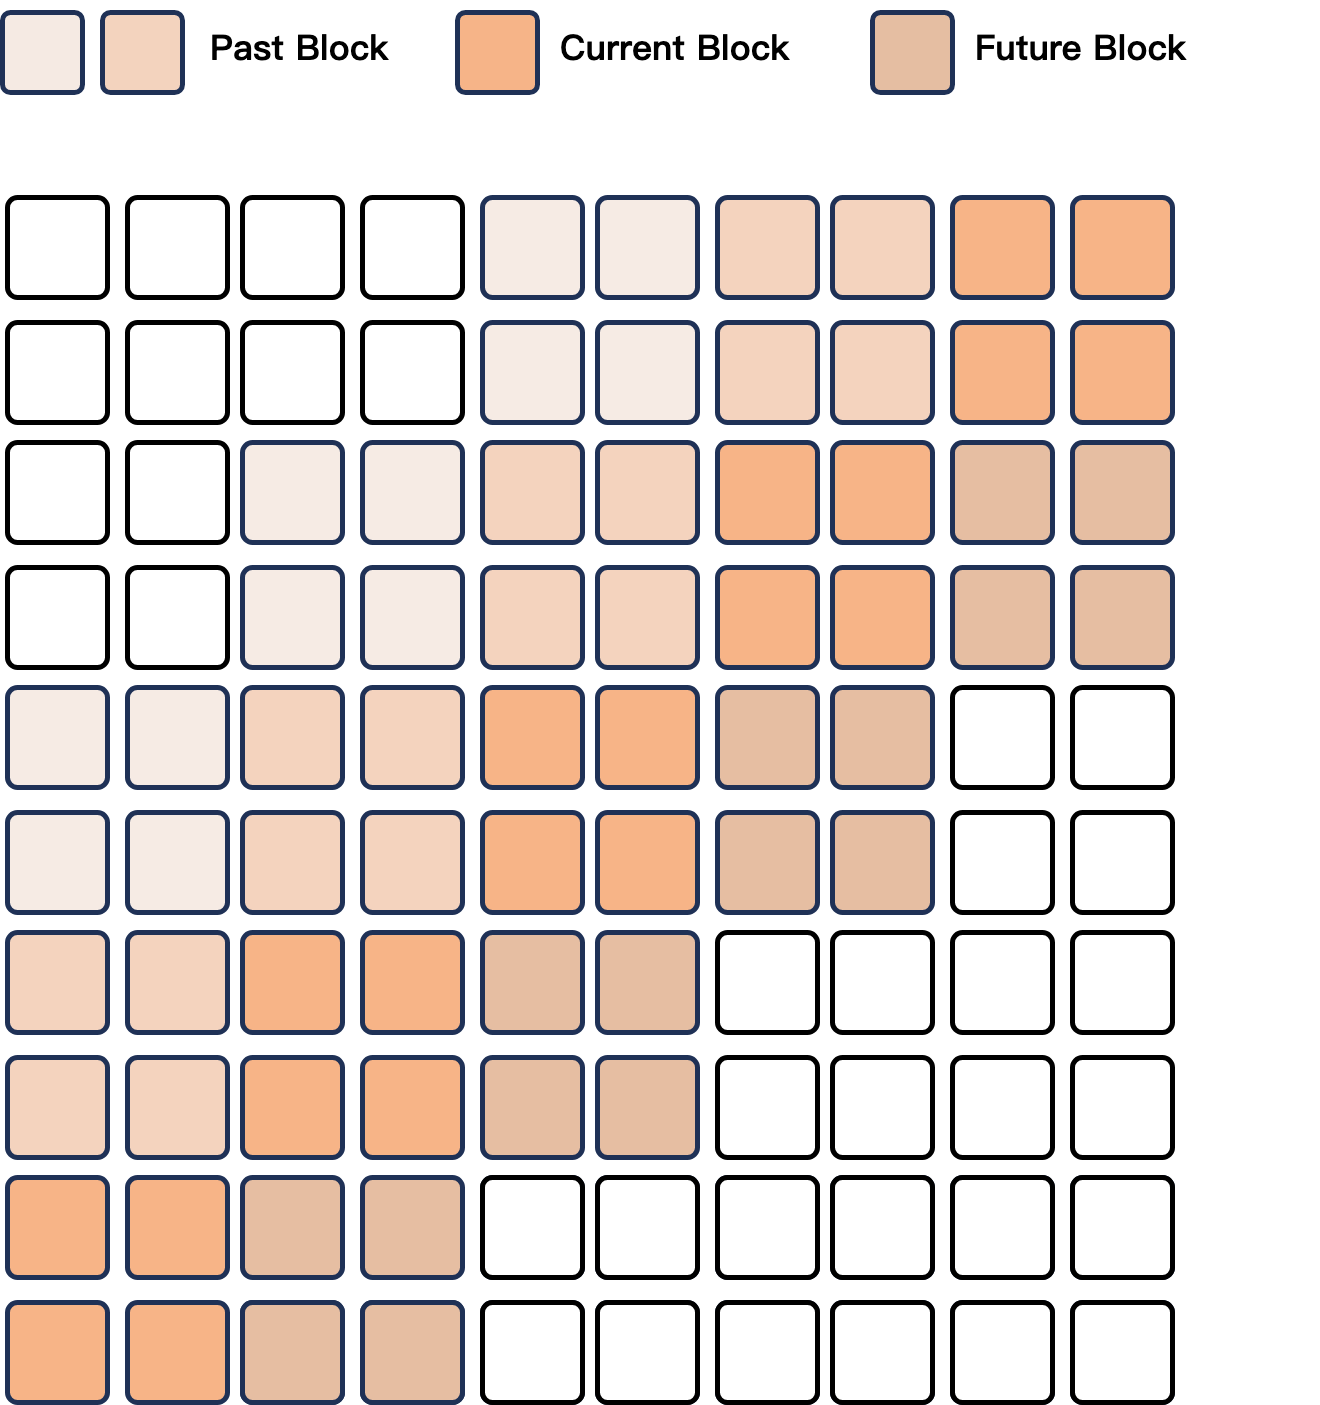
\includegraphics[width=0.3\textwidth]{figures/attentionmask.png}
    \caption{
An illustration of sliding window block attention mechanism in DiT for codec to wav generation.}
    \label{fig:attention_mask}
\end{figure}

As shown in Figure~\ref{fig:attention_mask}, to generate waveforms from code, we group adjacent codes into blocks and use these for our attention mask. We limit the DiT's receptive field to 4 blocks, including a lookback of 2 blocks and a lookahead of 1 block. During decoding, we generate the mel-spectrum in chunks using Flow Matching, ensuring that each code chunk has access to the necessary contextual blocks. This approach enhances the quality of streaming outputs by maintaining contextual information. We also use this chunk-by-chunk method for BigVGAN's fixed receptive field to facilitate streaming waveform generation

% \paragraph{Large Thinker and Small Talker.} To reduce the computational cost and latency, we use a small Talker, xxx M.


% For tokenization, we utilize Qwen's tokenizer~\citep{qwen}, which implements byte-level byte-pair encoding (BBPE,~\citealp{gpt3,wang2020neural,sennirch2016neural}) with a vocabulary of 151,643 regular tokens. We have expanded the set of control tokens from 3 to 22 compared to previous Qwen versions, adding two new tokens for tool functionality and allocating the remainder for other model capabilities. This expansion establishes a unified vocabulary across all Qwen2.5 models, enhancing consistency and reducing potential compatibility issues.

% \begin{table}[tbp]
% \caption{Model architecture and license of Qwen2.5 open-weight models.}
% \small
% \centering
% \begin{tabular}{@{}lcccccccc@{}} 
% \toprule
% Models  & Layers & Heads (Q / KV) & Tie Embedding & Context / Generation Length  & License \\
% \midrule
% 0.5B  & 24 & 14 / 2 & Yes & 32K / 8K & Apache 2.0 \\
% 1.5B  & 28 & 12 / 2 & Yes & 32K / 8K & Apache 2.0 \\
% 3B  & 36 & 16 / 2 & Yes & 32K / 8K & Qwen Research \\
% 7B  & 28 & 28 / 4 & No & 128K / 8K & Apache 2.0 \\
% 14B & 48 & 40 / 8 & No & 128K / 8K & Apache 2.0 \\
% 32B & 64 & 40 / 8 & No & 128K / 8K & Apache 2.0 \\
% 72B  & 80 & 64 / 8 & No & 128K / 8K & Qwen \\
% \bottomrule
% \end{tabular}
% \end{table}
